% 图 8.18 铁磁体自旋劈裂态密度示意：左多数自旋(↑) d 带填满于 E_F 下，右少数自旋(↓) d 带顶越过 E_F
\documentclass[tikz,border=5pt]{standalone}
\usetikzlibrary{arrows.meta}
\usepackage{amsmath}
\usepackage{bm}
\usepackage{fontspec}
\setmainfont{Times New Roman}
\begin{document}
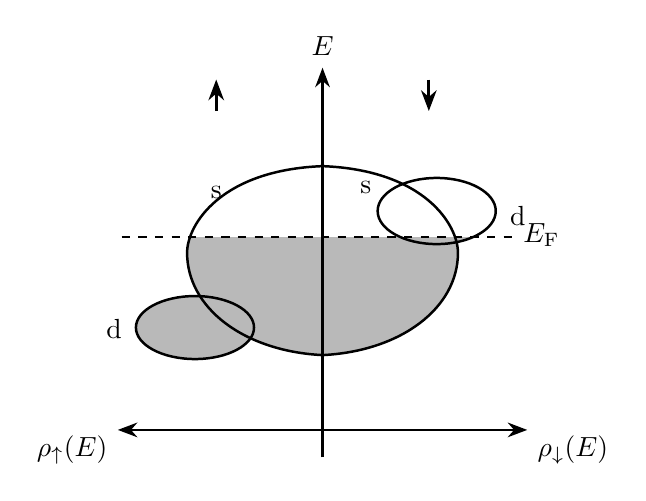
\begin{tikzpicture}[line width=0.8pt,>=Stealth]
% E_F level
\def\EF{0.45}
% ---------- occupied (below E_F) shading, clipped ----------
\begin{scope}
  \clip (-2.75,-2.45) rectangle (2.75,\EF);
  \fill[gray!55]
    (0,1.35) .. controls (-1.3,1.3) and (-1.72,0.6) .. (-1.72,0.25)
             .. controls (-1.72,-0.45) and (-1.0,-1.0) .. (0,-1.05) -- cycle;
  \fill[gray!55] (-1.62,-0.7) ellipse [x radius=0.75, y radius=0.40];
  \fill[gray!55]
    (0,1.35) .. controls (1.3,1.3) and (1.72,0.6) .. (1.72,0.25)
             .. controls (1.72,-0.45) and (1.0,-1.0) .. (0,-1.05) -- cycle;
  \fill[gray!55] (1.45,0.78) ellipse [x radius=0.75, y radius=0.42];
\end{scope}
% ---------- band outlines (drawn on top) ----------
\draw[line width=0.9]
  (0,1.35) .. controls (-1.3,1.3) and (-1.72,0.6) .. (-1.72,0.25)
           .. controls (-1.72,-0.45) and (-1.0,-1.0) .. (0,-1.05);
\draw[line width=0.9] (-1.62,-0.7) ellipse [x radius=0.75, y radius=0.40];
\draw[line width=0.9]
  (0,1.35) .. controls (1.3,1.3) and (1.72,0.6) .. (1.72,0.25)
           .. controls (1.72,-0.45) and (1.0,-1.0) .. (0,-1.05);
\draw[line width=0.9] (1.45,0.78) ellipse [x radius=0.75, y radius=0.42];
% ---------- E_F dashed line ----------
\draw[dashed,line width=0.7] (-2.55,\EF) -- (2.45,\EF);
\node[anchor=west] at (2.42,\EF+0.02) {$E_{\mathrm{F}}$};
% ---------- density-of-states axes ----------
\draw[->,line width=0.9] (0,-2.0) -- (-2.6,-2.0);
\draw[->,line width=0.9] (0,-2.0) -- (2.6,-2.0);
\node[anchor=east] at (-2.6,-2.25) {$\rho_{\uparrow}(E)$};
\node[anchor=west] at (2.6,-2.25) {$\rho_{\downarrow}(E)$};
% ---------- energy axis ----------
\draw[->,line width=0.9] (0,-2.35) -- (0,2.6);
\node[anchor=south] at (0,2.62) {$E$};
% ---------- labels ----------
\node at (-1.35,1.02) {s};
\node at (0.55,1.08) {s};
\node[anchor=east] at (-2.42,-0.72) {d};
\node[anchor=west] at (2.25,0.72) {d};
% ---------- spin arrows at the top ----------
\draw[->,line width=1.0] (-1.35,2.05) -- (-1.35,2.45);
\draw[->,line width=1.0] (1.35,2.45) -- (1.35,2.05);
\end{tikzpicture}
\end{document}
